\documentclass{report}

\usepackage[T2A]{fontenc}
\usepackage[utf8]{inputenc}
\usepackage[russian]{babel}

\usepackage{misccorr}
\usepackage{indentfirst}

\usepackage{setspace}
\onehalfspace

\usepackage{graphicx}

\usepackage{listings}
\lstset{captionpos=b}

\usepackage{amsmath}

\begin{document}

\tableofcontents

\chapter*{Введение}
\addcontentsline{toc}{chapter}{Введение}

В различных областях науки и техники довольно часто встречается
задача определения схожести строк. Например, набранные вручную
документы могут содержать опечатки, требующие исправления. Другой
пример: полученные с помощью телекоммуникации данные могут
содержать различные искажения из-за помех на линии. Для решения
подобных задач применяют разнообразные метрики схожести строк,
одними из которых являются расстояния Левенштейна и
Дамерау-Левенштейна.

\chapter{Аналитическая часть}

Расстояние Левенштейна определяется как минимальное количество
редакционных операций, необходимых для превращения одной строки в
другую.

Под редакционными операциями здесь понимают следующие действия над
строками:

\begin{itemize}
    \item вставка одного символа;
    \item удаление одного символа;
    \item замена одного символа на другой.
\end{itemize}

Расстояние Левенштейна между строками $\textbf{s}$ и $\textbf{t}$
длинами $m$ и $n$ соответственно может быть вычислено как
$d_{\textup{Л}}(m, n)$, где

\begin{equation} \label{eq:vl}
    d_{\textup{Л}}(i, j) =
    \begin{cases}
        0, i = 0, j = 0;
        \\
        j, i = 0, j > 0;
        \\
        \min
        \begin{cases}
            d_{\textup{Л}}(i, j - 1) + 1,
            \\
            d_{\textup{Л}}(i - 1, j) + 1,
            \\
            d_{\textup{Л}}(i - 1, j - 1) + \delta(i, j).
        \end{cases}
    \end{cases}
\end{equation}

Здесь и далее

$$
\delta(i, j) =
\begin{cases}
    \textup{если $\textbf{s}_i = \textbf{t}_j$, то }
    0;
    \\
    \textup{иначе }
    1.
\end{cases}
$$

В свою очередь, расстояние Дамерау-Левенштейна учитывает то
обстоятельство, что наиболее частой ошибкой при наборе человеком
текстов на клавиатуре является перестановка (транспозиция) двух
символов. Таким образом, под редакционными операциями здесь
понимают более широкий набор действий над строками:

\begin{itemize}
    \item вставка одного символа;
    \item удаление одного символа;
    \item замена одного символа на другой;
    \item перестановка двух символов.
\end{itemize}

Расстояние Дамерау-Левенштейна между строками $\textbf{s}$ и
$\textbf{t}$ длинами $m$ и $n$ соответственно может быть вычислено
как $d_{\textup{ДЛ}}(m, n)$, где

\begin{equation} \label{eq:dl}
    d_{\textup{ДЛ}}(i, j) =
    \begin{cases}
        0, i = 0, j = 0;
        \\
        j, i = 0, j > 0;
        \\
        \textup{если $\gamma(i, j)$, то}
        \min
        \begin{cases}
            d_{\textup{ДЛ}}(i, j - 1) + 1,
            \\
            d_{\textup{ДЛ}}(i - 1, j) + 1,
            \\
            d_{\textup{ДЛ}}(i - 1, j - 1) + \delta(i, j),
            \\
            d_{\textup{ДЛ}}(i - 2, j - 2) + 2;
        \end{cases}
        \\
        \textup{иначе}
        \min
        \begin{cases}
            d_{\textup{Л}}(i, j - 1) + 1,
            \\
            d_{\textup{Л}}(i - 1, j) + 1,
            \\
            d_{\textup{Л}}(i - 1, j - 1) + \delta(i, j).
        \end{cases}
    \end{cases}
\end{equation}

Здесь

$$
\gamma(i, j) =
\begin{cases}
    i, j > 1;
    \\
    \textbf{s}_i = \textbf{t}_{j - 1};
    \\
    \textbf{s}_{i - 1} = \textbf{t}_j.
\end{cases}
$$

На практике расстояния Левенштейна и Дамерау-Левенштейна могут
быть найдены с помощью различных алгоритмов.

Цель данной работы -- изучить метод динамического программирования
на примере реализации алгоритмов поиска расстояний Левенштейна и
Дамерау-Левенштейна.

Для этого необходимо решить следующие задачи:

\begin{enumerate}
    \item изучить расстояния Левенштейна и Дамерау-Левенштейна;
    \item разработать алгоритмы поиска изученных расстояний;
    \item реализовать разработанные алгоритмы;
    \item выполнить оценку затрат реализаций алгоритмов по памяти;
    \item выполнить замеры процессорного времени работы реализаций;
    \item выполнить сравнительный анализ разработанных алгоритмов.
\end{enumerate}

\chapter{Конструкторская часть}

В ходе работы были разработаны следующие алгоритмы поиска
расстояний Левенштейна и Дамерау-Левенштейна:

\begin{itemize}
    \item алгоритмы поиска расстояния Левенштейна:
    \begin{itemize}
        \item нерекурсивный;
    \end{itemize}
    \item алгоритмы поиска расстояния Дамерау-Левенштейна:
    \begin{itemize}
        \item нерекурсивный;
        \item простой рекурсивный;
        \item рекурсивный с кэшем.
    \end{itemize}
\end{itemize}

\section{Поиск расстояния Левенштейна}

\subsection{Нерекурсивный алгоритм} \label{vl-iterative}

Пусть $\textbf{s}$ и $\textbf{t}$ -- строки из $m$ и $n$ символов
соответственно, тогда $D$ -- целочисленная матрица $(m + 1) \times
(n + 1)$ элементов, причём $d_{ij}$ -- расстояние Левенштейна между
срезами $(\textbf{s}_k | k \in [1; i - 1])$ и
$(\textbf{t}_k | k \in [1; j - 1])$.

Матрица $D$ может быть вычислена с помощью двух вложенных циклов.

TODO: схема алгоритма

\section{Поиск расстояния Дамерау-Левенштейна}

\subsection{Нерекурсивный алгоритм}

Аналогично нерекурсивному алгоритму поиска расстояния Левенштейна,
рассмотренному в подразделе \ref{vl-iterative}, был разработан
нерекурсивный алгоритм поиска расстояния Дамерау-Левенштейна.

TODO: схема алгоритма

\subsection{Простой рекурсивный алгоритм}

Расстояние Дамерау-Левенштейна также может быть найдено
непосредственно по формуле \ref{eq:dl} с помощью рекурсивной
функции.

TODO: схема алгоритма

\subsection{Рекурсивный алгоритм с кэшем}

Главная проблема простого рекурсивного алгоритма поиска расстояния
Дамерау-Левенштейна в том, что многие значения выражения
\ref{eq:dl} вычисляются повторно. Очевидным решением является
введение кэша в виде матрицы, подобной рассмотренной в подразделе
\ref{vl-iterative}, но допускающей <<отсутствие>> значения каждого
элемента.

TODO: схема алгоритма

\chapter{Технологическая часть}

\section{Средства разработки}

Для реализации разработанных алгоритмов был выбран язык
программирования Rust, поскольку он предоставляет высокую степень
контроля за ошибками во время компиляции.

Также для разработки, тестирования и отладки программ был
использован инструмент Cargo, поскольку он позволяет
автоматизировать значительную часть работы.

Для замера процессорного времени был выбран крейт cpu-time,
поскольку он предоставляет простой и идиоматичный интерфейс.

\section{Реализация алгоритмов}

Далее представлен листинг реализации нерекурсивного алгоритма
поиска расстояния Левенштейна.

\begin{lstlisting}[caption=
    Нерекурсивная реализация алгоритма поиска расстояния
    Левенштейна.
]
fn distance(s: &str, t: &str) -> usize {
    let (m, n) = (s.len(), t.len());

    // A matrix of Levenshtein distances
    let mut matrix = Matrix::new(0, m + 1, n + 1);

    for i in 0..m + 1 {
        for j in 0..n + 1 {
            if i == 0 {
                matrix.set(0, j, j);
                continue;
            }

            if j == 0 {
                matrix.set(i, 0, i);
                continue;
            }

            // The current characters
            let c = s.chars().nth(i - 1).unwrap();
            let d = t.chars().nth(j - 1).unwrap();

            let mut cases = vec![matrix.get(i - 1, j - 1)
                + if c == d { 0 } else { 1 }];

            cases.push(matrix.get(i - 1, j) + 1);
            cases.push(matrix.get(i, j - 1) + 1);

            matrix.set(i, j, *cases.iter().min().unwrap());
        }
    }

    *matrix.get(m, n)
}
\end{lstlisting}

В свою очередь, листинг нерекурсивного алгоритма поиска расстояния
Дамерау-Левенштейна имеет следующий вид.

\begin{lstlisting}[caption=
    Нерекурсивная реализация алгоритма поиска расстояния
    Дамерау-Левенштейна.
]
fn distance(s: &str, t: &str) -> usize {
    let (m, n) = (s.len(), t.len());

    // A matrix of Damerau-Levenshtein distances
    let mut matrix = Matrix::new(0, m + 1, n + 1);

    for i in 0..m + 1 {
        for j in 0..n + 1 {
            if i == 0 {
                matrix.set(0, j, j);
                continue;
            }

            if j == 0 {
                matrix.set(i, 0, i);
                continue;
            }

            // The current characters
            let c = s.chars().nth(i - 1).unwrap();
            let d = t.chars().nth(j - 1).unwrap();

            let mut cases = vec![matrix.get(i - 1, j - 1)
                + if c == d { 0 } else { 1 }];

            cases.push(matrix.get(i - 1, j) + 1);
            cases.push(matrix.get(i, j - 1) + 1);

            if i > 1 && j > 1 {
                // The previous characters
                let p = s.chars().nth(i - 2).unwrap();
                let q = t.chars().nth(j - 2).unwrap();

                if c == q && p == d {
                    cases.push(matrix.get(i - 2, j - 2) + 1);
                }
            }

            matrix.set(i, j, *cases.iter().min().unwrap());
        }
    }

    *matrix.get(m, n)
}
\end{lstlisting}

Листинг простой рекурсивной реализации алгоритма поиска расстояния
Дамерау-Левенштейна демонстрирует наглядность такого подхода.

\begin{lstlisting}[caption=
    Простая рекурсивная реализация алгоритма поиска расстояния
    Дамерау-Левенштейна.
]
fn distance(s: &str, t: &str) -> usize {
    let (m, n) = (s.len(), t.len());

    if m == 0 {
        return n;
    }

    if n == 0 {
        return m;
    }

    // The last characters
    let c = s.chars().nth(m - 1).unwrap();
    let d = t.chars().nth(n - 1).unwrap();

    let mut cases = vec![Self::distance(&s[..m - 1], &t[..n - 1])
        + if c == d { 0 } else { 1 }];

    cases.push(Self::distance(&s[..m - 1], t) + 1);
    cases.push(Self::distance(s, &t[..n - 1]) + 1);

    if m > 1 && n > 1 {
        // The last but one characters
        let p = s.chars().nth(m - 2).unwrap();
        let q = t.chars().nth(n - 2).unwrap();

        if c == q && p == d {
            cases.push(Self::distance(&s[..m - 2], &t[..n - 2]) + 1);
        }
    }

    *cases.iter().min().unwrap()
}
\end{lstlisting}

\section{Тестирование}

\begin{lstlisting}[caption=Тесты алгоритмов поиска расстояния Левенштейна]
// Both strings are empty
assert_eq!(distance("", ""), 0);

// The first string is empty
assert_eq!(distance("", "right"), 5);

// The second string is empty
assert_eq!(distance("left", ""), 4);

// One insertion is required
assert_eq!(distance("word", "world"), 1);

// One deletion is required
assert_eq!(distance("clock", "lock"), 1);

// One replacement is required
assert_eq!(distance("ping", "pong"), 1);

// One transposition is required
assert_eq!(distance("vse", "sve"), 2);

// Both strings are the same
assert_eq!(distance("zug", "zug"), 0);

// Both strings are different
assert_eq!(distance("heaven", "hell"), 4);
\end{lstlisting}

\begin{lstlisting}[caption=Тесты реализаций алгоритмов поиска расстояния Дамерау-Левенштейна]
// Both strings are empty
assert_eq!(distance("", ""), 0);

// The first string is empty
assert_eq!(distance("", "right"), 5);

// The second string is empty
assert_eq!(distance("left", ""), 4);

// One insertion is required
assert_eq!(distance("word", "world"), 1);

// One deletion is required
assert_eq!(distance("clock", "lock"), 1);

// One replacement is required
assert_eq!(distance("ping", "pong"), 1);

// One transposition is required
assert_eq!(distance("vse", "sve"), 1);

// Both strings are the same
assert_eq!(distance("zug", "zug"), 0);

// Both string are different
assert_eq!(distance("heaven", "hell"), 4);
\end{lstlisting}

\chapter{Экспериментальная часть}

\section{Замеры процессорного времени}

Были проведены замеры процессорного времени работы реализации
каждого алгоритма. Полученные данные представлены в виде графиков.

\begin{figure}[ht]
    \centering
    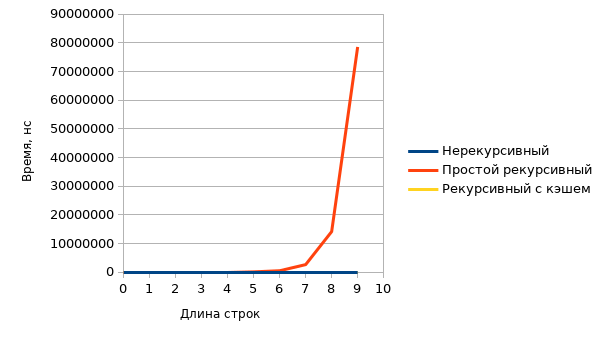
\includegraphics[width=\textwidth]{plt-01.png}
    \caption{Сравнение времени работы реализаций трёх алгоритмов}
\end{figure}

\begin{figure}[ht]
    \centering
    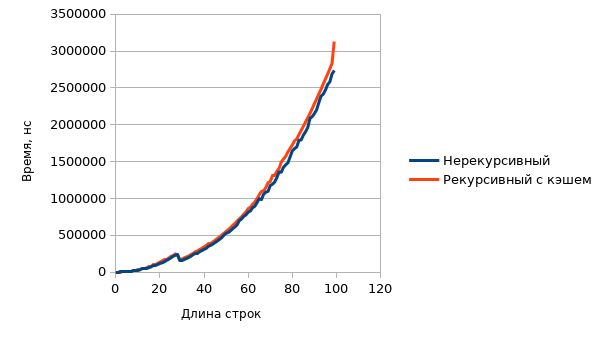
\includegraphics[width=\textwidth]{plt-02.png}
    \caption{Сравнение времени работы реализаций двух алгоритмов}
\end{figure}

\section{Выводы}

\chapter*{Заключение}
\addcontentsline{toc}{chapter}{Заключение}

В ходе работы были решены следующие задачи:

\begin{enumerate}
    \item изучены расстояния Левенштейна и Дамерау-Левенштейна;
    \item разработаны алгоритмы поиска изученных расстояний;
    \item реализованы разработанные алгоритмы;
    \item выполнены оценки затрат реализаций алгоритмов по памяти;
    \item выполнены замеры процессорного времени работы реализаций;
    \item выполнен сравнительный анализ следующих алгоритмов:
    \begin{itemize}
        \item нерекурсивного поиска расстояния Левенштейна и
            нерекурсивного поиска расстояния Дамерау-Левенштейна;
        \item поиска расстояния Дамерау-Левенштейна;
    \end{itemize}
\end{enumerate}

TODO: выводы

\chapter*{Список литературы}
\addcontentsline{toc}{chapter}{Список литературы}

1. Левенштейн, В. И. Двоичные коды с исправлением выпадений,
вставок и замещений символов. / В. И. Левенштейн // Доклады
Академий Наук СССР. -- 1965. -- 163.4. -- 845-848.

2. Damerau, F. J. A technique for computer detection and correction
of spelling errors. / F. J. Damerau // Communications of the ACM.
-- 1964. -- 7 (3). -- 171-176.

\end{document}
